\documentclass[tikz,border=6pt]{standalone}
\usepackage{amsmath}
\usetikzlibrary{arrows.meta, calc, fit}

\definecolor{lincol}{RGB}{244, 206, 206}
\definecolor{rffcol}{RGB}{214, 205, 238}
\definecolor{normcol}{RGB}{173, 197, 238}
\definecolor{attncol}{RGB}{157, 199, 132}
\definecolor{ffcol}{RGB}{246, 232, 185}
\definecolor{framecol}{RGB}{230, 134, 112}
\definecolor{plaincol}{RGB}{248, 248, 248}

\begin{document}
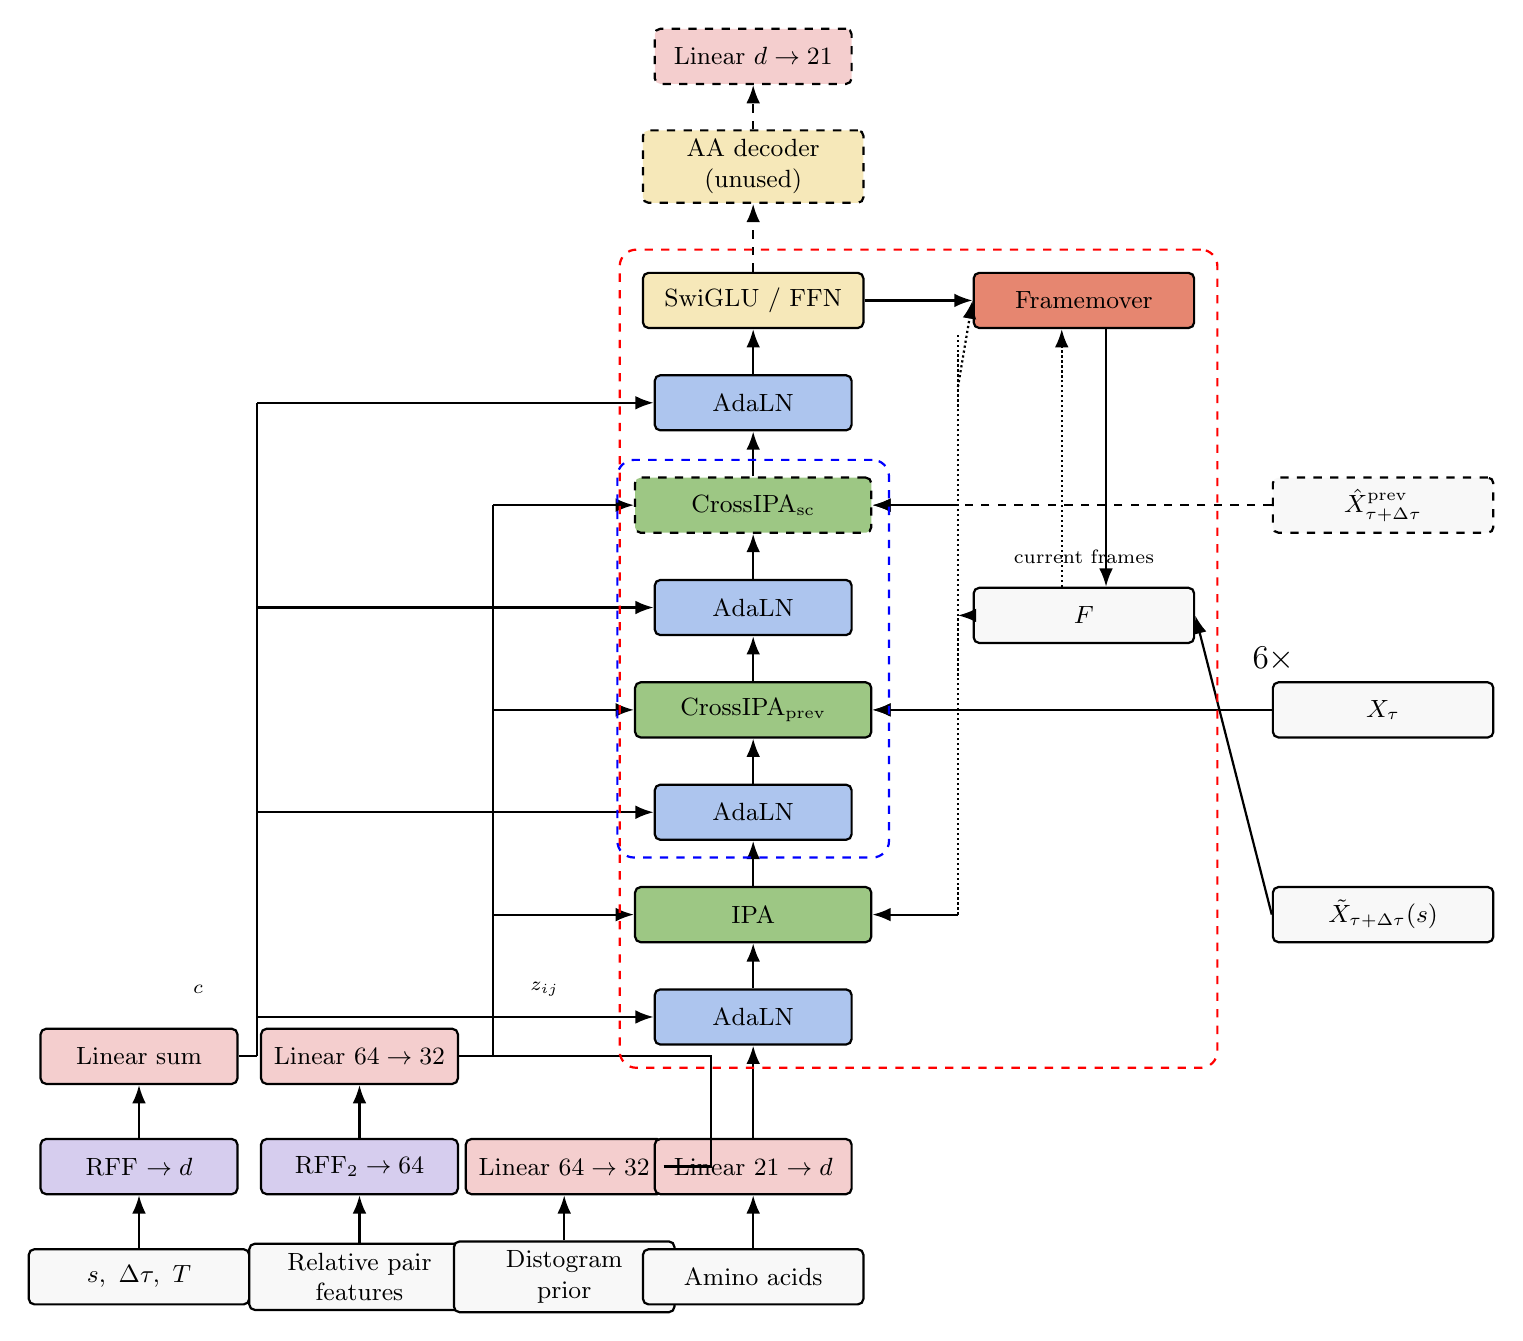
\begin{tikzpicture}[
    >=Latex,
    font=\small,
    flow/.style={-Latex, thick},
    optflow/.style={-Latex, thick, dashed},
    wire/.style={thick},
    framewire/.style={densely dotted, thick},
    box/.style={draw, rounded corners=2pt, thick, minimum height=7mm, align=center},
    linbox/.style={box, fill=lincol, minimum width=25mm},
    rffbox/.style={box, fill=rffcol, minimum width=25mm},
    normbox/.style={box, fill=normcol, minimum width=25mm},
    attnbox/.style={box, fill=attncol, minimum width=30mm},
    ffbox/.style={box, fill=ffcol, minimum width=28mm},
    framebox/.style={box, fill=framecol, minimum width=28mm},
    plainbox/.style={box, fill=plaincol, minimum width=28mm},
    tinylabel/.style={font=\scriptsize}
]

% Bottom inputs and encoders
\node[plainbox] (flowin) at (-6.4,-10.0) {$s,\ \Delta\tau,\ T$};
\node[rffbox]   (flowrff) at (-6.4,-8.6) {RFF $\to d$};
\node[linbox]   (flowlin) at (-6.4,-7.2) {Linear sum};

\node[plainbox] (pairbase) at (-3.6,-10.0) {Relative pair\\features};
\node[rffbox]   (pairrff)  at (-3.6,-8.6) {RFF$_2 \to 64$};
\node[linbox]   (pairlin)  at (-3.6,-7.2) {Linear $64 \to 32$};

\node[plainbox] (disto)    at (-1.0,-10.0) {Distogram\\prior};
\node[linbox]   (distolin) at (-1.0,-8.6) {Linear $64 \to 32$};

\node[plainbox] (aas)      at (1.4,-10.0) {Amino acids};
\node[linbox]   (aaenc)    at (1.4,-8.6) {Linear $21 \to d$};

% Central stack
\node[normbox]  (adaln1)    at (1.4,-6.7) {AdaLN};
\node[attnbox]  (ipa)       at (1.4,-5.4) {IPA};
\node[normbox]  (adaln2)    at (1.4,-4.1) {AdaLN};
\node[attnbox]  (crossprev) at (1.4,-2.8) {CrossIPA$_{\mathrm{prev}}$};
\node[normbox]  (adaln3)    at (1.4,-1.5) {AdaLN};
\node[attnbox, dashed] (crosssc) at (1.4,-0.2) {CrossIPA$_{\mathrm{sc}}$};
\node[normbox]  (adaln4)    at (1.4,1.1)  {AdaLN};
\node[ffbox]    (ffn)       at (1.4,2.4)  {SwiGLU / FFN};

% Optional legacy head, shown only to match the original ChainStorm visual language
\node[ffbox, dashed]  (headff)  at (1.4,4.1)  {AA decoder\\(unused)};
\node[linbox, dashed] (headlin) at (1.4,5.5)  {Linear $d \to 21$};

% Frame state and movers
\node[framebox] (move)  at (5.6,2.4)  {Framemover};
\node[plainbox] (fbox)  at (5.6,-1.6) {$F$};

% External frame inputs
\node[plainbox]         (noisy) at (9.4,-5.4) {$\tilde{X}_{\tau+\Delta\tau}(s)$};
\node[plainbox]         (prevf) at (9.4,-2.8) {$X_{\tau}$};
\node[plainbox, dashed] (scf)   at (9.4,-0.2) {$\hat{X}^{\mathrm{prev}}_{\tau+\Delta\tau}$};

% Main vertical token stream
\draw[flow] (aas) -- (aaenc);
\draw[flow] (aaenc) -- (adaln1);
\draw[flow] (adaln1) -- (ipa);
\draw[flow] (ipa) -- (adaln2);
\draw[flow] (adaln2) -- (crossprev);
\draw[flow] (crossprev) -- (adaln3);
\draw[flow] (adaln3) -- (crosssc);
\draw[flow] (crosssc) -- (adaln4);
\draw[flow] (adaln4) -- (ffn);
\draw[optflow] (ffn) -- (headff);
\draw[optflow] (headff) -- (headlin);

% Conditioning bus into every AdaLN
\coordinate (condbus0) at (-4.9,-7.2);
\coordinate (condbus1) at (-4.9,1.1);
\draw[flow] (flowin) -- (flowrff);
\draw[flow] (flowrff) -- (flowlin);
\draw[wire] (flowlin.east) -- (condbus0);
\draw[wire] (condbus0) -- (condbus1);
\draw[flow] (condbus0 |- adaln1.west) -- (adaln1.west);
\draw[flow] (condbus0 |- adaln2.west) -- (adaln2.west);
\draw[flow] (condbus0 |- adaln3.west) -- (adaln3.west);
\draw[flow] (condbus0 |- adaln4.west) -- (adaln4.west);

% Pair-feature bus into every attention block
\coordinate (pairbus0) at (-1.9,-7.2);
\coordinate (pairbus1) at (-1.9,-0.2);
\draw[flow] (pairbase) -- (pairrff);
\draw[flow] (pairrff) -- (pairlin);
\draw[flow] (disto) -- (distolin);
\draw[wire] (pairlin.east) -- ++(0.6,0) |- (pairbus0);
\draw[wire] (distolin.east) -- ++(0.6,0) |- (pairbus0);
\draw[wire] (pairbus0) -- (pairbus1);
\draw[flow] (pairbus0 |- ipa.west) -- (ipa.west);
\draw[flow] (pairbus0 |- crossprev.west) -- (crossprev.west);
\draw[flow] (pairbus0 |- crosssc.west) -- (crosssc.west);
\node[tinylabel] at (-1.25,-6.35) {$z_{ij}$};

% Frame-state wiring
\coordinate (framewire0) at (4.0,-5.4);
\coordinate (framewire1) at (4.0,2.0);
\draw[framewire] (framewire0) -- (framewire1);
\draw[flow] (fbox.west) -- (4.0,-1.6);
\draw[flow] (framewire0 |- ipa.east) -- (ipa.east);
\draw[flow] (framewire0 |- crossprev.east) -- (crossprev.east);
\draw[flow] (framewire0 |- crosssc.east) -- (crosssc.east);
\draw[framewire, -Latex] (4.0,1.3) -- (move.west);
\draw[framewire, -Latex] ([xshift=-8pt]fbox.north) -- ([xshift=-8pt]move.south);
\draw[flow] ([xshift=8pt]move.south) -- ([xshift=8pt]fbox.north);
\draw[flow] (ffn.east) -- (move.west);

% External frame inputs
\draw[flow]    (noisy.west) -- (fbox.east);
\draw[flow]    (prevf.west) -- (crossprev.east);
\draw[optflow] (scf.west) -- (crosssc.east);

% Visual grouping to mimic the original ChainStorm architecture figure
\node[draw=red, dashed, rounded corners=6pt, thick, fit=(adaln1)(ffn)(move)(fbox), inner sep=8pt] (outer) {};
\node[draw=blue, dashed, rounded corners=6pt, thick, fit=(adaln2)(crossprev)(adaln3)(crosssc), inner sep=6pt] (inner) {};
\node[font=\large] at ($(outer.east)+(0.7,0)$) {$6\times$};

% Small labels for the buses
\node[tinylabel] at (-5.65,-6.35) {$c$};
\node[tinylabel] at (5.6,-0.85) {current frames};

\end{tikzpicture}
\end{document}
